Environment reconstruction is an active field of research, it has been studied by the computer vision, photogrammetry and robotics communities. A particularly successful approach to this problem is known as Simultaneous Localization and Mapping (SLAM). The task in SLAM is to estimate the position of an entity (robot, car, person) by the metrics provided by sensors and at the same time construct a map of the environment (Figure~\ref{fig:intro:slam})~\cite{Thrun2008_SLAM}.\\[0.1em]

\begin{figure}[hb]
  \begin{center}
    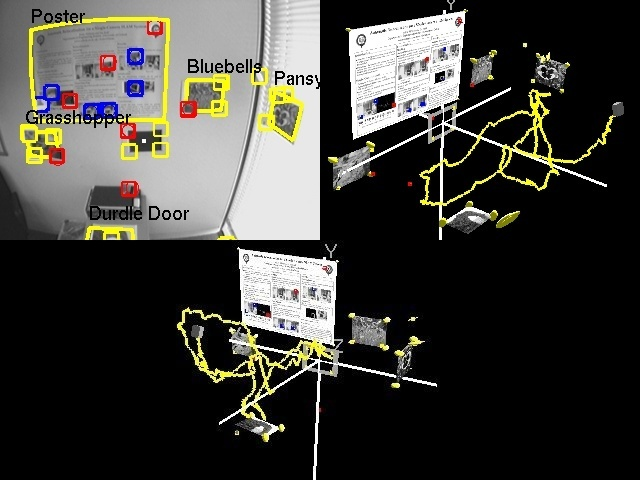
\includegraphics[width=0.65\textwidth]{slam-illustration-castle_etal_icra2007}
    \caption{The SLAM problem. From a series of sensed images (upper left corner), estimate the camera position (yellow lines) and recreate the scene (objects ``floating'')~\cite{slam-oxford-images}.}
    \label{fig:intro:slam}
  \end{center}
\end{figure}

%GPS unreliable because it's not precise, a couple of meters of difference could lead a car jumping on the curve or bumping another while trying to park.
Most research has cameras and/or a mixture of exotic depth sensors as inputs.
Depth sensors such as laser range finders are expensive, do not provide texture information and are bulky. That restricts mobile applications to vehicles where the cost of carrying such equipment is negligible (e.g. cars).
By operating only on visual input $visual$SLAM removes some of the restrictions, though cameras still stream large quantities of information which have to be processed. If a real-time solution is desired, the most probable scenario is to run the algorithms in power-hungry devices. This is something that limits the actual utility for mobile systems with limited power resources. 
%Another disadvantage to using ``classic'' computer vision approaches is that computational resources would need to be shared inefficiently (i.e. a processor would have to switch between a facial recognition algorithm to a depth-estimation one). Having a neuro inspired system means that the tasks are executed by the same network.

However, the human brain -- which only require $\sim 20 watt$ of power to operate -- performs this task all the time. This suggests that a neural approach to SLAM may be an energy-efficient means of solving the problem.
%Given that humans are able to do something similar with an efficient highly-parallel biological computing system that requires about 20-watts to function, our brain; we propose that a neural approach to SLAM is an energy-efficient way of solving the problem. The question of how exactly this is done in the brain is still open and is subject to research~\cite{rat-slam}. This work will provide a solution, inspired by state-of-the-art neuroscience, to the environment reconstruction problem using neuromorphic hardware.

General purpose hardware is inefficient for simulating large scale neural networks so, instead, we propose to use SpiNNaker -- a general purpose computing hardware platform inspired by the brain~\cite{furber2014spinnaker}. 
%If one is to develop a neural network based solution and remain power efficient, the best way to achieve this is on a neuromorphic processing platform. SpiNNaker provides a massively-parallel high-efficiency computing platform, inspired by the brain. 
%These characteristics make it an excellent choice for neuroscience research, particularly to study spiking neural networks~\cite{furber2014spinnaker}.
As well as using significantly less power than a conventional computer system~\cite{stromatias2013power}, SpiNNaker has the additional advantages of operating in real time and neuromorphic vision sensors.
Sensors which have shown to reduce representations so that irrelevant information is not transmitted nor processed~\cite{aer-retina-bernabe,dvs-zurich}.
